\section{Fonctionnement des failles}


Les deux failles utilisent le m\^eme principe et tiennent leur existence du fait que les anciennes versions des protocoles SSL/TLS comportent des failles. L'adversaire utilise une attaque de type "man in the middle" et force l'utilisation d'une version vulnérable de SSL, de manière à pouvoir exploiter ses failles. Parfois il n'est m\^eme pas utile de la forcer, car quand un navigateur doté d’une version récente n’arrive pas à se connecter à un serveur non mis à jour, ou mal configuré, il réessaie en utilisant des versions anciennes : c’est la downgrade dance, qui peut aboutir à l'utilisation d'une ancienne version vulnérable.

\subsection{Un point sur SSL/TLS}

\subsubsection{Historique}

SSL/TLS sont des protocoles qui fonctionnent suivant un mode client-serveur, et qui garantissent l'authentification du serveur et du client (optionnel), ainsi que la confidentialité et l'intégrité de données echangées. SSL est l'ancien nom de TLS, et a vécu sur 3 versions:
\begin{itemize}
\item 1994: SSL 1.0
\item Février 1995: SSL 2.0, première version réellement utilisée.
\item Novembre 1996: SSL 3.0 
\end{itemize}
TLS a ensuite pris le relais: 
\begin{itemize}
\item Janvier 1999: TLS 1.0
\item Avril 2006: TLS 1.1
\item Avril 2008: TLS 1.2
\end{itemize}
TLS, comme SSLv3, intègre un mécanisme de compatibilité ascendante avec les versions précédentes. Ainsi, quand le client et le serveur négocient la version du protocole qu'ils vont utiliser, ils peuvent choisir la plus récente commune aux deux. En Mars 2011, la compatibilité des versions TLS avec SSLv2 a été abandonnée. \\
La plupart des navigateurs supportent la version TLS 1.2:
\begin{itemize}
\item Google Chrome 30 et suivants
\item Mozilla Firefox 27 et suivants
\item Microsoft Internet Explorer 11 et suivants
\item Opera 17 et suivants
\item Apple Safari 7 et suivants
\end{itemize}
Plus précisément, TLS est composé de deux niveaux: TLS Record Protocol (couche transport) et TLS Handshake Protocol (couche session).

\subsubsection{TLS Handshake protocol}

Ce protocole permet l'authentification et l'échange de clés nécessaires pour établir une session sécurisée. La figure \ref{handshake} décrit les différentes étapes de ce protocole:
\begin{figure}[H]
  \centering
  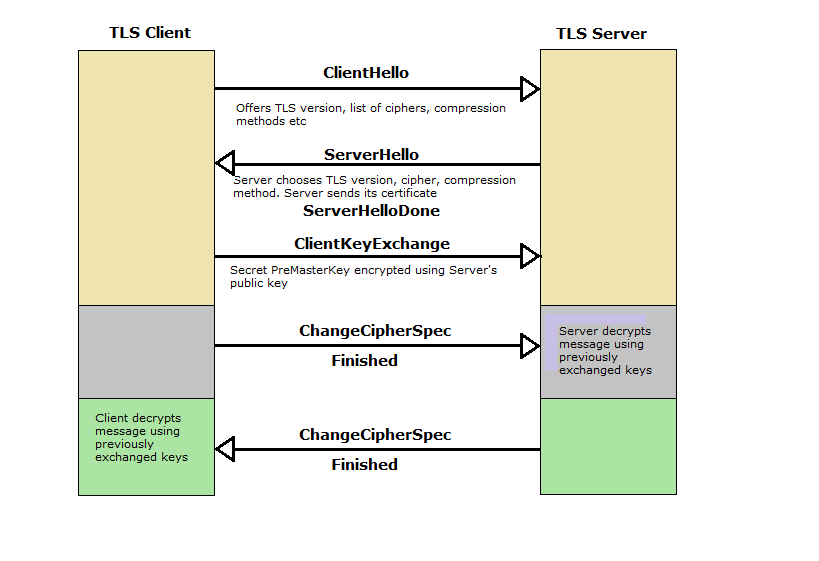
\includegraphics[scale=0.6]{img/tls-handshake.png}
  \caption{TLS handshake}
  \label{handshake}
\end{figure}  

Détails de chaque étape:
\begin{itemize}
\item le client envoie un message "ClientHello" au serveur, pour lui indiquer la dernière version TLS qu'il supporte, la liste des algorithmes de chiffrement qu'il supporte et les méthodes de compression qu'il supporte. Il envoie également un nombre aléatoire
\item le serveur renvoie un message "ServerHello", indiquant la version TLS, l'algorithme de chiffrement et la méthode de compression qui seront utilisés. Il envoie également son certificat (permettant l'authentification) et un nombre aléatoire
\item le serveur envoie un message "ServerHelloDone" pour indiquer qu'il a fini avec la première phase du handshake
\item le client génère un nombre appelé "PreMasterSecret", encrypté avec la clé publique du certificat du serveur
\item le client et le serveur génèrent alors leur secret partagé "Master Secret" à partir de leur nombre aléatoire et du "PreMasterSecret"
\item le client envoie un message "ChangeCipherSpec" indiquant que la suite de la communication sera cryptée, et envoie un message "Finished" qui est donc crypté
\item le serveur reçoit et décrypte le message et envoie son "ChangedCipherSpec"
\item le client reçoit et décrypte le message et c'est la fin du handshake
\end{itemize}
Les algorithmes utilisés pour l'échange de clés sont DH (Diffie-Hellman) et RSA. 

\subsubsection{TLS Record Protocol}

Ce protocole permet de sécuriser les données en utilisant les clés qu'on a crée pendant le handshake. Il permet également de vérifier l'intégrité des données. La figure \ref{record} présente son fonctionnement:
\begin{figure}[H]
\centering
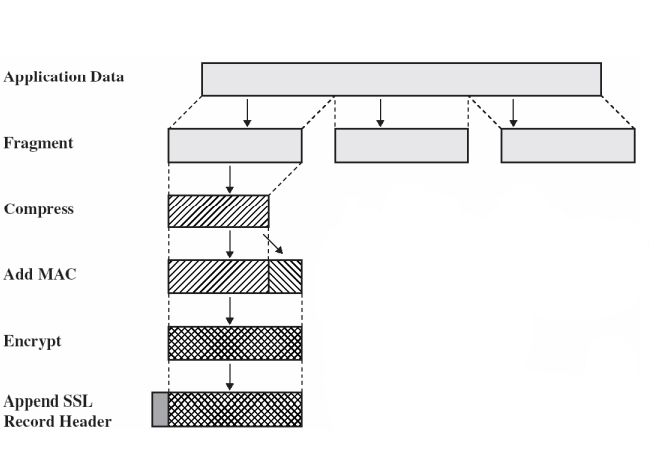
\includegraphics[scale=0.7]{img/tls-record.png}
\caption{TLS record}
\label{record}
\end{figure}

Détails des étapes:
\begin{itemize}
\item on divise le message à transmettre en fragments 
\item on compresse les fragments
\item on applique MAC (message authentification code) pour authentifier les messages 
\item on crypte les messages
\item on ajoute un en-t\^ete
\end{itemize}
Quand on reçoit un message, on fait l'opération inverse (décryptage, vérification d'authenfication avec le MAC, décompression, défragmentation). \\
Les algorithmes utilisés pour la phase de cryptage sont RC4, CBC, AES, DES, etc. \\

La sécurité du protocole est donc assurée par deux éléments:
\begin{itemize}
\item un chiffrement asymétrique qui permet, après authentification de la clé publique du serveur, la constitution d'un secret partagé entre le client et le serveur. C'est ce qui a lieu au cours du handshake
\item un chiffrement symétrique qui est utilisé dans la phase d'échange de données. C'est ce qui a lieu dans la phase de cryptage du record. Les clés de chiffrement symétrique sont calculées à partir du secret partagé (de plus, une fonction de hachage est également utilisée pour assurer l'intégrité et l'authentification des données)
\end{itemize}

La faille Poodle exploite une faiblesse de SSLv3 au niveau du chiffrement symétrique (CBC). \\
La faille Freak exploite une faiblesse de SSLv3 au niveau du chiffrement asymétrique (RSA).

\subsection{La faille Poodle}

Comme on le voit sur la figure \ref{poodle}, le principe est que le client demande un service qui nécessite l'utilisation de SSL/TLS, et l'adversaire, en utilisant une attaque de type "man in the middle", force l'utilisation de SSLv3 et exploite ses failles.

\begin{figure}[H]
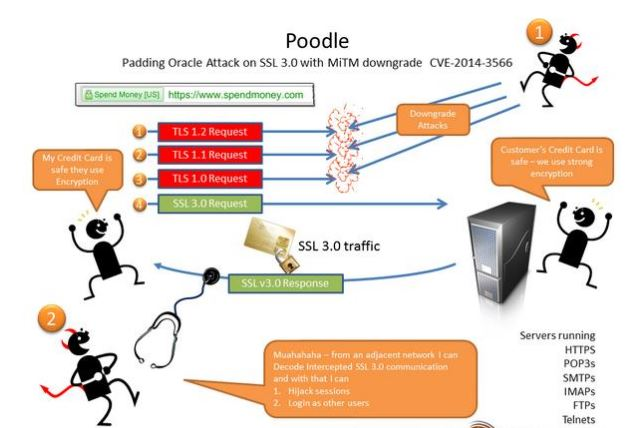
\includegraphics[scale=0.8]{img/poodle.jpg}
\caption{fonctionnement de la faille poodle}
\label{poodle}
\end{figure}

Avec cette méthode, l'adversaire n’a pas accès aux fichiers stockés dans l’appareil ciblé, mais il peut intercepter ses données de connexion, comme par exemple les cookies déposés dans le navigateur par un serveur lors d’une session. Sans posséder le mot de passe du client, l'adversaire peut effectuer des actions comme envoyer des messages sur Twitter en se faisant passer pour elle, lire et effacer son courrier électronique, etc.

\subsubsection{Détails de la vulnérabilité de SSLv3 exploitée}

Deux méthodes de chiffrement sont utilisées dans SSLv3:
\begin{itemize}
\item la première est RC4 (Rivest Cipher 4) qui est un chiffrement par flot (stream cipher). Le principe d'un chiffrement par flot est de générer un flot de bits aléatoires $k$ et de réaliser un XOR entre ce flot et le message à chiffrer $m$. L'avantage est que chiffrement et déchiffrement sont très rapides: si $c = m \oplus k$, alors $m = c \oplus k$. Cependant, RC4 est actuellement considéré comme peu s\^ur et ne devrait plus \^etre utilisé
\item l'autre méthode est un chiffrement par blocs cha\^inés (CBC pour cipher block chaining), et c'est elle qui fait l'objet de l'attaque Poodle que l'on va détailler
\end{itemize}

\paragraph{Fonctionnement du chiffrement par blocs cha\^inés}

Les chiffrements et déchiffrements par blocs cha\^inés sont illustrés en figure \ref{cbc-enc} et \ref{cbc-dec} (Plaintext est le message en clair noté $m$ et Ciphertext est le message chiffré noté $c$) \\

\noindent On utilise la formule suivante pour chiffrer: \\
$c_i = Enc_K(m_i \oplus c_{i-1}),\ c_0 = IV$

\begin{figure}[H]
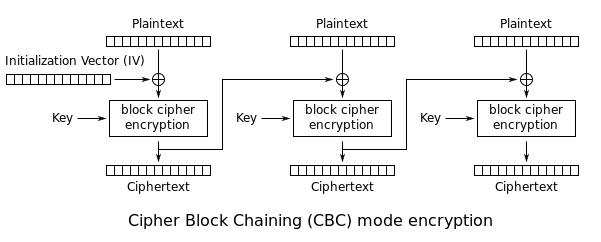
\includegraphics[scale=0.6]{img/cbc-enc.png}
\caption{CBC encryption}
\label{cbc-enc}
\end{figure}

\noindent On utilise la formule suivante pour déchiffrer: \\
$m_i = Dec_K(c_i) \oplus c_{i-1},\ c_0 = IV$ 

\begin{figure}[H]
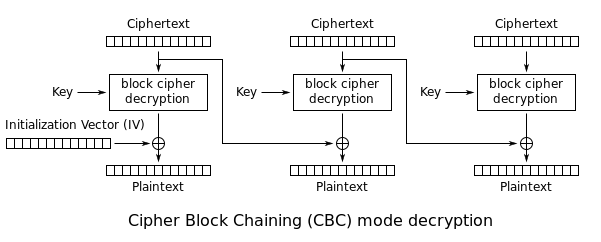
\includegraphics[scale=0.6]{img/cbc-dec.png}
\caption{CBC decryption}
\label{cbc-dec}
\end{figure}

Si un bit du message chiffré change, le bloc de message en clair correspondant est complètement corrompu et cela inverse le bit correspondant dans le bloc suivant de message en clair, mais le reste du bloc ne change pas. C'est ce qui est exploité par Poodle.

Supposons que l'adversaire ait trois blocs chiffrés $c_1$, $c_2$ et $c_3$ et qu'il souhaite décrypter le second bloc (et donc obtenir $m_2$). Il sait seulement que le dernier bloc est complété (padded) en utilisant la méthode PKCS7, c'est à dire que le dernier bloc est complété avec $n$ octets, chacun égal à $n$.
Le décryptage fonctionne comme ceci: $m_i = Dec(c_i) \oplus c_{i-1}$, avec $c_0 = IV$. Si l'adversaire change le dernier octet de $c_1$ et envoie ($IV$, $c_1$, $c_2$) au serveur, cela va affecter tout le bloc $m_1$ et le dernier octet de $m_2$. Ensuite le serveur va vérifier le dernier bloc décrypté ($m_2$) et retourner oui ou non si la complétion ("padding") est correcte.
Si $b_{-1}$ est le dernier octet de $c_1$, l'adversaire le change comme suit: $b_{-1} = b_{-1} \oplus z_{-1} \oplus$ 0x01, où $z_{-1}$ est la valeur du dernier octet de $m_2$. Si $z_{-1}$ est correct, le serveur ne va pas trouver d'erreur de padding (parce que le dernier octet de $m_2$ sera égal à 0x01, ce qui est un padding correct). Dans l'autre cas, le serveur va trouver une erreur de padding et l'adversaire va essayer une autre valeur de $z_{-1}$. Dans le pire des cas, il doit faire 255 essais pour trouver la bonne valeur de $z_{-1}$.

Une fois qu'il connait le dernier octet de $m_2$, l'adversaire peut obtenir l'avant dernier octet de $m_2$. Il change les deux derniers octets de $c_1$: $b_{-1} = b_{-1} \oplus z_{-1} \oplus$ 0x02 et $b_{-2} = b_{-2} \oplus z_{-2} \oplus$ 0x02. Après 255 essais au maximum il trouve $z_{-2}$ et ainsi de suite. 

Si chaque bloc fait 128 bits (AES), soit 16 octets, l'adversaire va obtenir $m_2$ en moins de 255x16 = 4080 essais. Cette attaque ne co\^ute presque rien et peut \^etre réalisée en quelques secondes.

La publication de Google qui a officialisé le faille offre les détails nécessaires pour récupérer les cookies d'une cible: This POODLE Bites: Exploiting The SSL 3.0 Fallback, Security Advisory, Bodo Möller, Thai Duong, Krzysztof Kotowicz, Google, September 2014.


\subsection{La faille Freak}


